\chapter{Ablation Study Visualisations}
\label{appendix:ablation_study_visualisations}

\section{Question Processing Module Ablations}
\label{section:question_processing_module_ablation_visualisations}

As described in \subsectionautorefname{ \ref{subsec:question_module_ablations}}, the BiLSTM question module performed poorly on compare-type questions compared to the GAT question module. In \figureautorefname{ \ref{fig:question_ablation_sample}}, we see an example image with a corresponding binary comparison question. For this sample, the model that used the GAT question module answered the question correctly, where the one that used the BiLSTM question module answered incorrectly. In \figureautorefname{ \ref{fig:bilstm_gat_control_attention_maps}}, we see that the attended question features for the GAT question module are much more appropriate than those for the BiLSTM question module; the GAT question module attends to phrases like \textit{have the same color} in the second reasoning step, \textit{as the pants} in the third reasoning step and \textit{the skis} in the final reasoning step. Conversely, the BiLSTM question module attends to the words \textit{do} in reasoning steps 1, 2 and 3, and attends to \textit{skis} in the final reasoning step. The attended question features for the BiLSTM and GAT question modules are reflected in the read unit attentions shown in \figureautorefname{ \ref{fig:bilstm_read_attention_maps}} and \figureautorefname{ \ref{fig:gat_read_attention_maps}} respectively.

\begin{figure}[htbp]
    \centering
    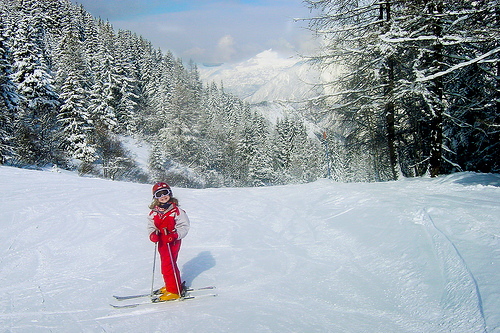
\includegraphics[width=0.5\textwidth]{figures/qav/skipants.png}
    \caption[A sample compare-type question and its correponding image.]{\textit{Do the skis have the same color as the pants ?} \textbf{No}}
    \label{fig:question_ablation_sample}
\end{figure}

\begin{figure}[htbp]
    \centering
    \begin{subfigure}[l]{0.5\textwidth}
        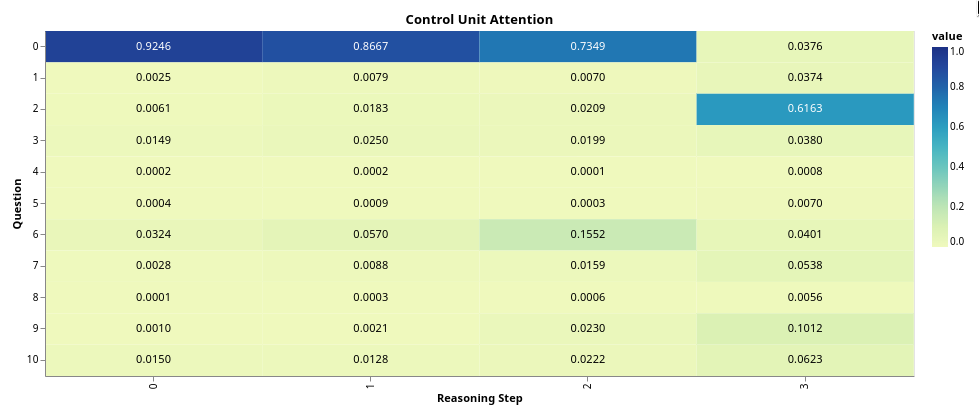
\includegraphics[width=\textwidth]{figures/qav/qav_cu.png}
        \caption{BiLSTM question module attention map.}
    \end{subfigure}
    \begin{subfigure}[r]{0.49\textwidth}
        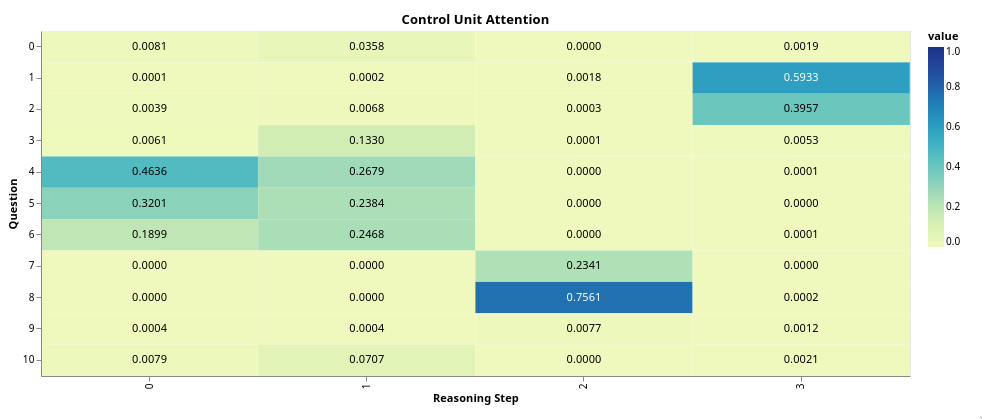
\includegraphics[width=\textwidth]{figures/qav/qav_gat_cu.png}
        \caption{GAT question module attention map.}
    \end{subfigure}
    \caption[Control unit attention maps for BiLSTM and GAT question processing modules.]{Control unit attention maps for a BiLSTM question module and a GAT question module given the question \textit{Do the skis have the same color as the pants ?}}
    \label{fig:bilstm_gat_control_attention_maps}
\end{figure}


\begin{figure}[htbp]
    \centering
    \begin{subfigure}[l]{0.4\textwidth}
        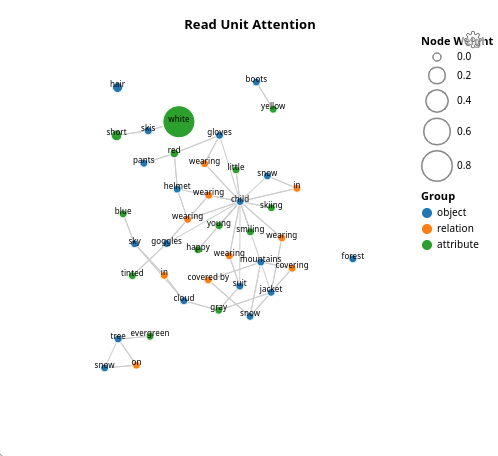
\includegraphics[width=\textwidth]{figures/qav/qav_r0.png}
        \caption{Reasoning step 1}
    \end{subfigure}
    \begin{subfigure}[r]{0.4\textwidth}
        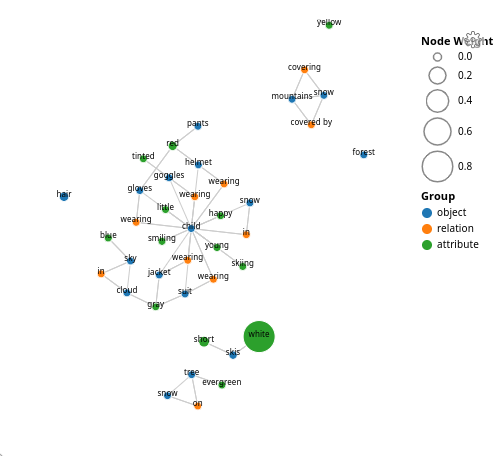
\includegraphics[width=\textwidth]{figures/qav/qav_r1.png}
        \caption{Reasoning step 2}
    \end{subfigure}
    \begin{subfigure}[l]{0.4\textwidth}
        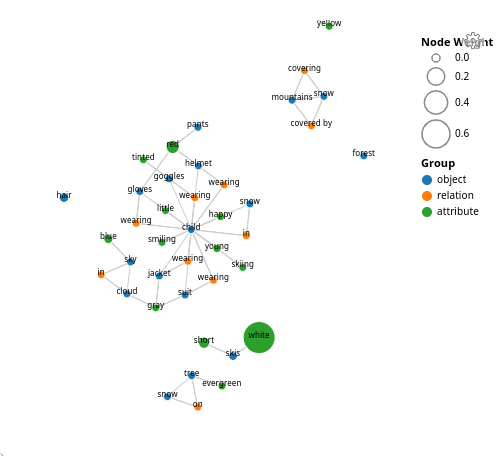
\includegraphics[width=\textwidth]{figures/qav/qav_r2.png}
        \caption{Reasoning step 3}
    \end{subfigure}
    \begin{subfigure}[r]{0.4\textwidth}
        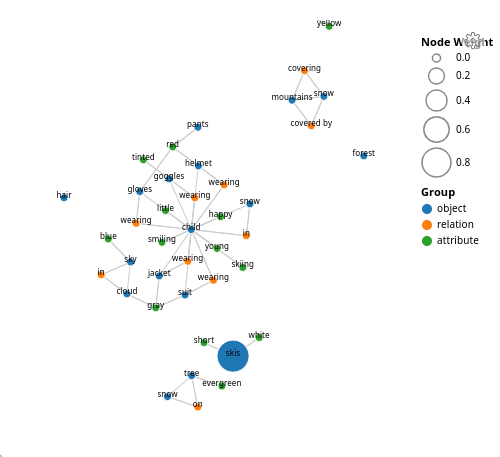
\includegraphics[width=\textwidth]{figures/qav/qav_r3.png}
        \caption{Reasoning step 4}
    \end{subfigure}
    \caption[A collection of BiLSTM question module read unit attemtion maps]{Read unit attention maps at each reasoning step for the model that uses a BiLSTM question module given the question \textit{Do the skis have the same color as the pants ?}. Across all reasoning steps, the main information extracted from the scene graph is the colour of the skis, which is not enough information to answer the question correctly.}
    \label{fig:bilstm_read_attention_maps}
\end{figure}

\begin{figure}[htbp]
    \centering
    \begin{subfigure}[l]{0.4\textwidth}
        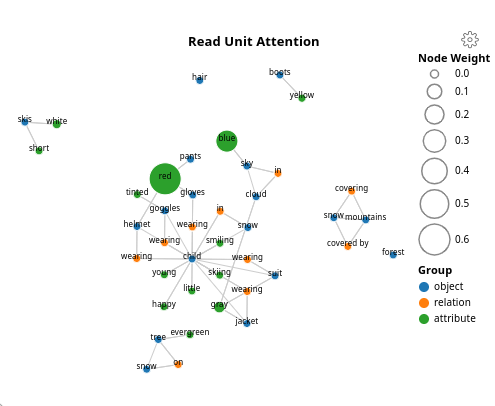
\includegraphics[width=\textwidth]{figures/qav/qav_gat_r0.png}
        \caption{Reasoning step 1}
    \end{subfigure}
    \begin{subfigure}[r]{0.4\textwidth}
        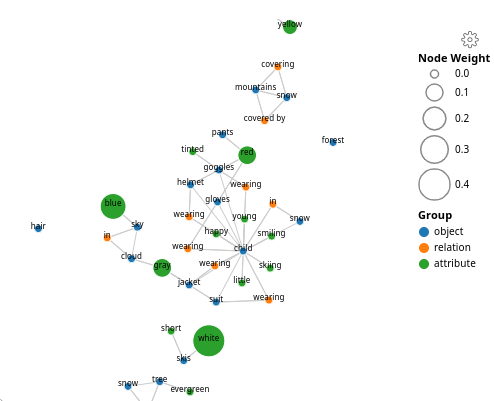
\includegraphics[width=\textwidth]{figures/qav/qav_gat_r1.png}
        \caption{Reasoning step 2}
    \end{subfigure}
    \begin{subfigure}[l]{0.4\textwidth}
        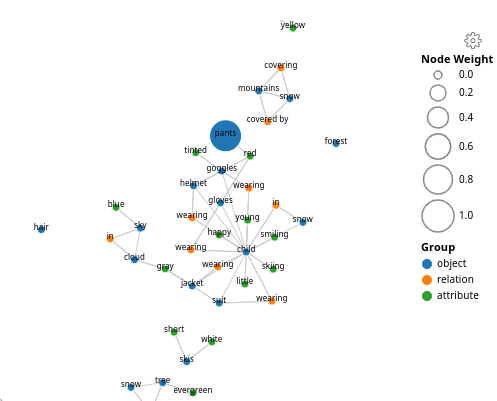
\includegraphics[width=\textwidth]{figures/qav/qav_gat_r2.png}
        \caption{Reasoning step 3}
    \end{subfigure}
    \begin{subfigure}[r]{0.4\textwidth}
        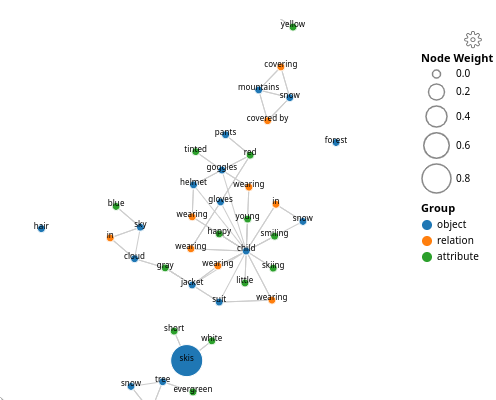
\includegraphics[width=\textwidth]{figures/qav/qav_gat_r3.png}
        \caption{Reasoning step 4}
    \end{subfigure}
    \caption[A collection of GAT question module read unit attemtion maps]{Read unit attention maps at each reasoning step for the model that uses a GAT question module given the question \textit{Do the skis have the same color as the pants ?} In the first and second reasoning steps, the model attends to relevant colour attributes in the scene graph, before attending to the pants in the third reasoning step and finally the skis.}
    \label{fig:gat_read_attention_maps}
\end{figure}
